The carefully chosen set of target platforms have great impact on
the design of the proposed toolchain. This will remain so in the future as we further refine the
design environment---particularly the feedback mechanisms from the
deployment stages. Based on our
initial experience with various platforms, we recognize two
fundamentally different computational models in the task scheduling
and communication domains. We believe that many of the practical
distributed embedded environments can be described by a
combination and blending of these models.

Event-triggered (ET) real-time systems are driven solely by the
occurrence of various events, e.g. the reception of a message, the
assertion of an external interrupt line, or a timeout. In this
computational model, the system responds to these events as
soon as possible, resulting in a very flexible but highly
unpredictable environment. A notable purely event-triggered distributed embedded platform is TinyOS \cite{tinyos}.

In stark contrast to event-triggered systems, time-triggered (TT)
systems generate control signals with the progression of a
system-wide global time over a static schedule defined in
the design phase. These control signals might trigger the sending
and receiving of messages, the activation of application tasks, or
mode changes.

One of the most important conclusions we reached in the early stages
of the project was to separate the communication models and task
scheduling models on the target platforms. This enabled us to mix
and match these approaches and provided the flexibility to
characterize real-world embedded execution platforms. The
interactions between these models and domains are an interesting and
important research area \cite{ucb:ptolemy2}; however, in the
prototype version of the proposed toolchain, we focused on the time-triggered scheduling and communication aspects of the target
platforms.

Although these platforms differ in their implementation of the time-triggered approach---later sections will detail these
differences---all follow some general rules and use similar
concepts. We support a general TT component model in the modeling
language we developed, called ECSL-DP. According to the TT model,
the timeline (both in the
communication and task scheduling domains) is divided into continuously
repeating periods. The task and message schedule describe the
partitioning of this period. The length of the periods for task
scheduling and for communication are of equal length but obviously
have different partitioning. Optionally, the period can be divided
into subperiods of equal lengths (hardware implementations of TTA function in this way). Both the communication
subsystem and task scheduler wait for the beginning of the
period---in a synchronized manner---and control access to the
communication medium and/or release tasks according to a predefined
schedule throughout the period. At the end of the period, the whole
process starts again.

\subsubsection{The Time-Triggered Architecture platform}

One of the experimental target platforms for the toolchain is the
Time Triggered Architecture \cite{kopetz:2001-22} developed at the
Vienna University of Technology and by TTTech Computertechnik AG.
The primary reasons for selecting TTA, in general, and the
TTP-Development Cluster as a test platform were its fault-tolerance features, performance characteristics, and its technological maturity.

Fault-tolerance is supported by redundant communication channels, by
replicated subsystems with constant state synchronization and
voting in the value domain, and by various provisions in the
communication protocol (e.g. cluster startup, distributed time
synchronization, and membership management with clique avoidance). The
measured jitter, relatively high bandwidth, and protocol efficiency (low overhead)
are definitely superior to
similar performance metrics measured in general purpose (ET)
computer systems. However, one of the most crucial advantages of the Time-Triggered Platform (TTP)
for the system designer lies in its composability aspects. A
well-designed cluster schedule (with enough spare capacity for
future growth) guarantees that existing services are not affected by
the removal or the addition of other services both in the value and time domains. Furthermore, due to the dedicated and
autonomous protocol controller, these changes are transparent to the
application level software. Also, for similar reasons, application
level errors are not propagated to other nodes and do not disrupt
the communication channels.

These characteristics made the TTA platform and TTP prime targets for the proposed toolchain . On the other
hand, we faced various constraints and peculiarities inherent
in the TTP protocol, some of which had profound effects on the system
design and on the design environment. These lessons confirmed the need for an integrated environment,
where (late) deployment decisions are able to influence the (early)
design phases via feedback in the toolchain. This section gives a
brief overview of the protocol to illustrate some of the special
characteristics of TTP and their effects on the system
design.

In TTP all protocol operations, except during the \emph{startup}
phase, are initiated at \emph{a priori} known points in time. All
nodes that are integrated in the cluster agree on a global time. This
requires synchronized clocks with a fault-tolerant
synchronization protocol. The global clock is defined in a
\emph{sparse time base}, in which granularity is limited by the
precision of the distributed clock synchronization. The granularity
factor ($\Pi$) is an important parameter in the system design and
depends on the accuracy of the local oscillators, the frequency of
the synchronization points (TTP does not use skew compensation
techniques), on the speed of the communication controller, and the
physical medium. The communication controller has complete knowledge
of the message schedule---defined in a special descriptor table
located in the memory of the controller---and provides a shared
memory interface for the host processor to access the messages to be
sent and received.

The message schedule defines a \emph{cluster cycle}---or multiple
cluster cycles if cluster mode changes are allowed---which is
executed periodically (see Figure~\ref{fig:TTPSchedule}). The
cluster cycle is further divided into \emph{TDMA rounds}. Within a
TDMA round each node is assigned to exactly one slot---a time
interval where it can send messages packed into a single frame on
the communication bus. The length of these slots may differ for
different nodes, but they are constant throughout the TDMA rounds in the
cluster cycle (thus the length of the TDMA rounds are of the same
length in the cycle). Mode changes may alter the length of the
cluster cycle (the number of rounds in a cycle) and the message
contents of the frames, but the same ordering and lengths
of the time slots for the nodes should be used. These spartan scheduling rules make
mode changes and scheduling more deterministic and easier to handle,
but they have crucial effects on the system design. In a typical TTP
application, the length of the TDMA rounds are around 1-2~ms and the
precision of the synchronization is below 5~$u$S (re-synchronization
occurs at the end of each round). However, the number of rounds in a cycle
varies substantially, as do the length and contents of the frames.

\begin{figure}[h]
   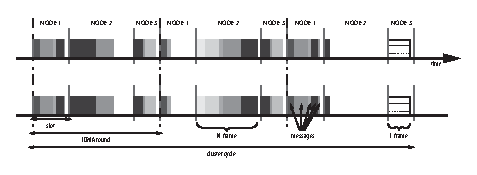
\includegraphics[width=3in]{TTPSchedule}
   \caption{Message scheduling in a TTP application.}
   \label{fig:TTPSchedule}
\end{figure}

The application design on the TTP platform may follow two different
approaches. In the simpler case, the application level tasks are not
synchronized to the communication bus, and tasks access the messages via
the shared memory interface as they wish. This approach has obvious
limitations (no guarantees on end-to-end jitter and latency) and can
hardly be considered real-time. More interesting is the second
alternative, where application tasks are activated in sync with the
message schedule. To support this method, the communication
controller provides interrupts to the host processor at well-defined
time instants while executing the protocol. The real-time operating
system running on the host processor is able to align the task
schedule with the bus schedule. Evidently, the limitations on the
message schedule affect the task schedule also in these systems. The
application cycle has to follow (match in its length) the cluster
cycle. Also, tasks cannot be released before the arrival of their
input message(s) and must finish before the transmission of their
output(s). Furthermore, fault management for subsystem replication
(tolerance against faults in the value domain) is implemented as
higher level services running on the host processor, thus additional
tasks and their dependencies have to be considered in the
application design. The task schedule with its important
dependencies in a typical application is shown in
Figure~\ref{fig:TTPAppSchedule}.

\begin{figure}[h]
\begin{center}
   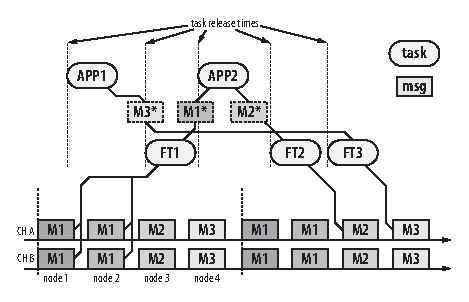
\includegraphics[width=3in]{TTPAppSchedule}
   \caption{Message scheduling in a TTP application.}
   \label{fig:TTPAppSchedule}
\end{center}
\end{figure}